
\section{Introduction}
\label{sec:introduction}

\begin{figure}[t]
    \centering
    % \subfloat[\label{fig:fpn_vis} \textbf{Strong correlation} between feature scales in feature pyramids and object sizes.]
    % {
    %     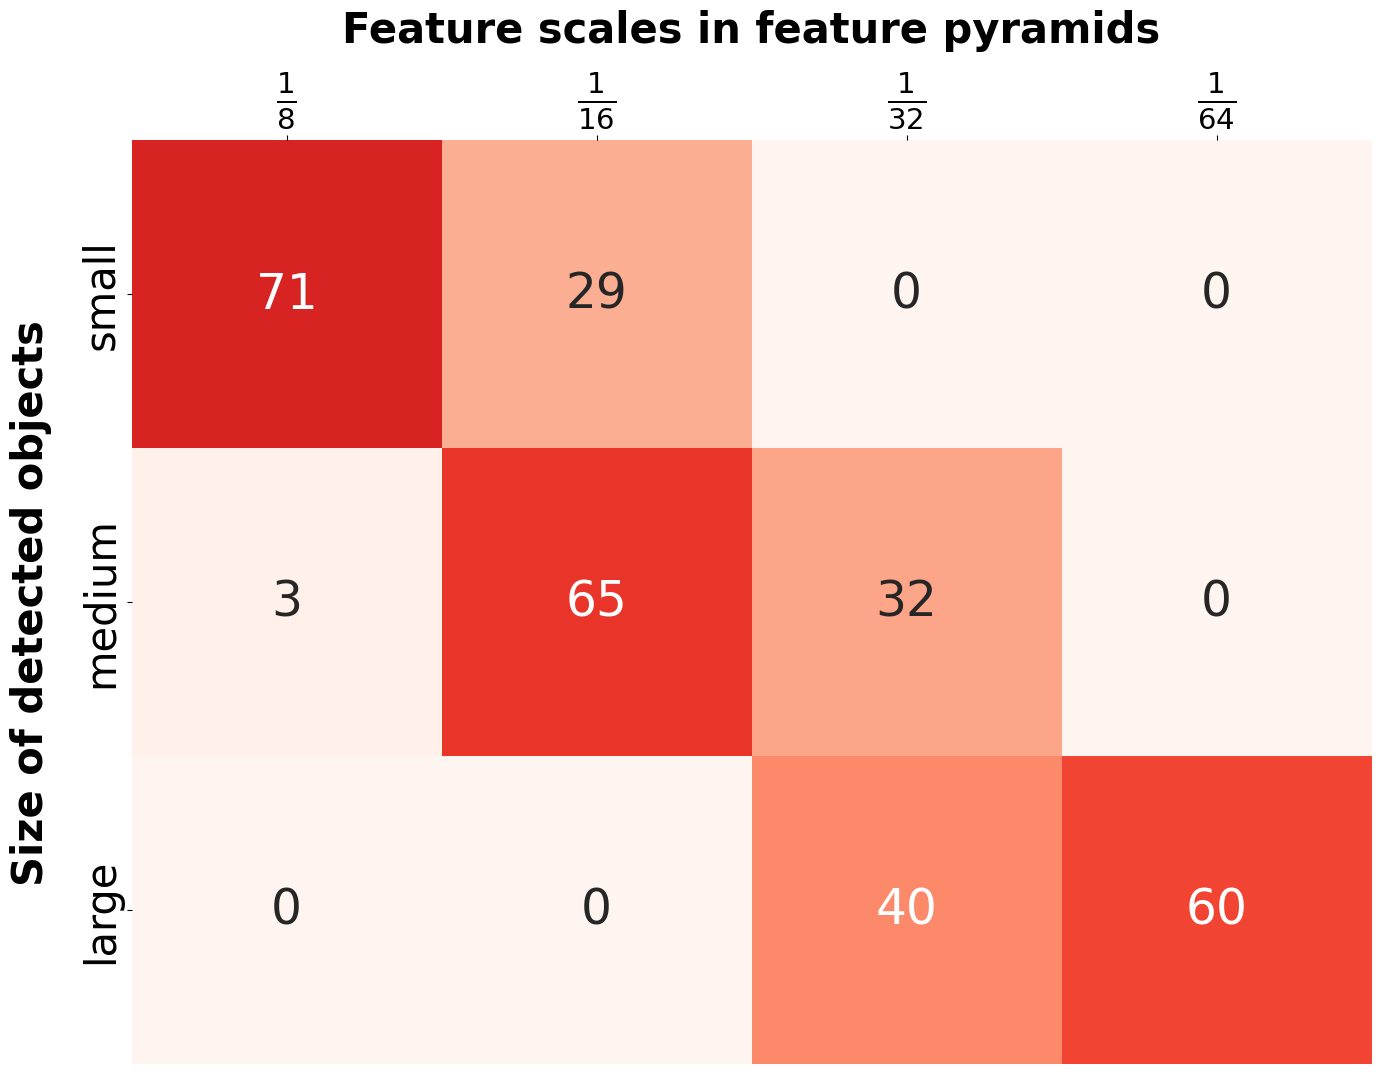
\includegraphics[width=\linewidth]{fig/fpn_vis.png}
    % }
    % \subfloat[\label{fig:fpn_comp} \textbf{Feature pyramids are important}, showing a considerable improvement over single-scale input in current detectors.]
    {
        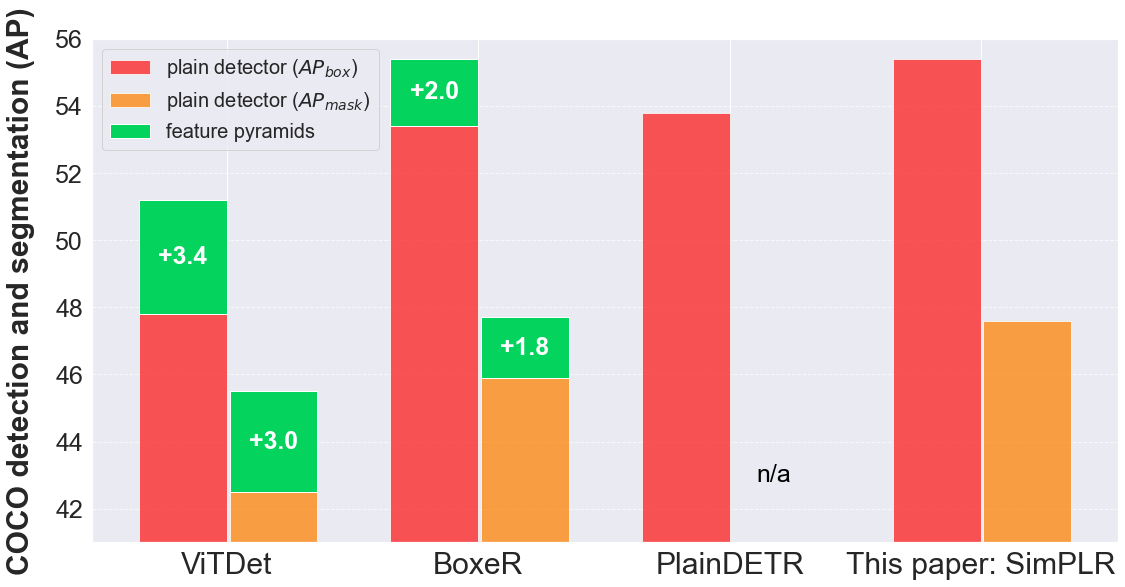
\includegraphics[width=\linewidth]{fig/fpn_comp.png}
    }
    \caption{
    \textbf{A plain detector is non-trivial.} Even with the use of a plain backbone ViT pre-trained using MAE~\cite{he2022mae}, feature pyramids are still important for both convolution-based (ViTDet~\cite{li2022vitdet}) and transformer-based (BoxeR~\cite{nguyen2022boxer}) detectors. While removing multi-scale input from the encoder, PlainDETR~\cite{lin2023plaindetr} still relies on feature pyramids for its box proposal generation and lags behind in performance. In this paper, we demonstrate that the plain detector, \ours, with the proposed scale-aware attention yields competitive performance compared to multi-scale counterparts. %(n/a: PlainDETR is for object detection only).
    }\label{fig:single_scale}
\end{figure}

% \footnotetext{In this paper, ``plain'' refers to the non-hierarchical, single-scale property. The ``plain detector'' is the detector whose backbone and detection head are non-hierarchical and both operate on single-scale features.}

After its astonishing achievements in natural language processing, the transformer \citep{vaswani2017transformer} has quickly become the neural network architecture of choice in computer vision, as evidenced by recent success in image classification \citep{liu2021swintransformer,dosovitskiy2021vit}, object detection \citep{nicolas2020detr,zhu2021deformable,nguyen2022boxer} and segmentation \citep{wang2021maxdeeplab,zhang2021knet,cheng2022mask2former}. Unlike natural language processing, where the same pre-trained network can be deployed for a wide range of downstream tasks with only minor modifications \citep{brown2020gpt3,devlin2019bert}, computer vision tasks such as object detection and segmentation require a different set of domain-specific knowledge to be incorporated into the network. Consequently, it is commonly accepted that a modern object detector contains two main components: a pre-trained backbone as the \emph{general} feature extractor, and a \emph{task-specific} head that conducts detection and segmentation tasks using domain knowledge. For transformer-based vision architectures, the question remains whether to add more inductive biases or to learn them from data.

The spatial nature of image data lies at the core of computer vision. Besides learning long range feature dependencies, the ability of capturing local structure of neighboring pixels is critical for representing and understanding the image content. Building upon the successes of convolutional neural networks, a line of research biases the transformer architecture to be \emph{multi-scale} and \emph{hierarchical} when dealing with the image input, \ie, Swin Transformer \cite{liu2021swintransformer} and others \citep{fan2021mvit,wang2021pvit,heo2021rethinkingvit}.
The hierarchical design makes it easy to create multi-scale features for dense vision tasks and allows pre-trained transformers to be seamlessly integrated into a convolution-based detection head with a feature pyramid network \citep{tsung2017fpn}, yielding impressive results in object detection and segmentation. However, the inductive biases in the architectural design make it benefit less from self-supervised learning and the scaling of model size~\citep{li2022vitdet}.

An alternative direction pursues the idea of a simple transformer with ``less inductive biases'' and emphasizes learning vision-specific knowledge directly from image data. 
Specifically, the Vision Transformer (ViT) \citep{dosovitskiy2021vit} stands out as a \emph{plain} architecture with a constant feature resolution, and acts as the feature extractor in plain-backbone detection. This is motivated by the success of ViTs scaling behaviours in visual recognition \citep{he2022mae,bao2022beit,dehghani2023scalingvit22b}. In addition, the end-to-end detection framework proposed by Carion \etal \cite{nicolas2020detr} with a transformer-based detection head further removes many hand-designed components, like non-maximum suppression or intersection-over-union computation, that encodes the prior knowledge for object detection. 

The plain design of ViTs, however, casts doubts about its ability to capture information of objects across multiple scales. While recent studies \citep{dosovitskiy2021vit,li2022vitdet} suggest that ViTs with global self-attention could potentially learn translation-equivariant and scale-equivariant properties during training, leading object detectors still require multi-scale feature maps and/or an hierarchical backbone. This observation holds true for both convolutional \citep{ren2015faster_rcnn,he2017maskrcnn,li2022vitdet} and transformer-based detectors \citep{zhu2021deformable,nguyen2022boxer,cheng2022mask2former} (see \cref{fig:single_scale}). Unlike hierarchical backbones, the creation of feature pyramids conflicts with the original design philosophy of ViTs. Therefore, our goal is to pursue a plain detector whose backbone \textit{and} detection head are both \textit{single-scale} and \textit{non-hierarchical}. This further simplifies the architecture for detection and segmentation in the pursuit of learning object representations from data.

In this paper, we introduce SimPLR, a plain detector for \textit{both} end-to-end detection and segmentation frameworks~\cite{nicolas2020detr,zhu2021deformable,nguyen2022boxer,cheng2022mask2former}. In particular, our detector extracts the single-scale feature map from a ViT backbone, which is then fed into the transformer encoder-decoder via a simple projection to make the prediction. To deal with objects of various sizes, we propose to incorporate scale information into the attention mechanism, resulting in an \emph{adaptive-scale} attention. The proposed attention mechanism learns to capture adaptive scale distribution from training data. This eliminates the need for multi-scale feature maps from the ViT backbone, yielding a simple and efficient detector.

The proposed detector, \ours, turns out to be an effective solution for the plain detection and segmentation. We find that multi-scale feature maps are not necessary and the scale-aware attention mechanism adequately captures objects at various sizes from output features of a ViT backbone. Despite the plain architecture, our detector (\ours) shows competitive performance compared to the strong hierarchical-backbone or multi-scale detectors (\eg, ViTDet~\cite{li2022vitdet} and Mask2Former~\cite{cheng2022mask2former}), while being consistently faster. Moreover, the effectiveness of our detector is observed not only in object detection but also in instance and panoptic segmentation. Interestingly, the efficient design allows \ours to take advantages of the significant progress in self-supervised learning and scaling with ViTs (\eg, with MAE~\cite{he2022mae} and BEiT~\cite{peng2022beitv2}), indicating plain detectors to be a promising direction for dense prediction tasks.